% Change the size of math notation inside math environment(Problem occurs in line 257): https://tex.stackexchange.com/questions/348108/change-the-size-of-a-math-symbol

% Page transitions-> \transwipe[duration=0.6], \transdissolve, \transblindshorizontal, \transblindsvertical, \transboxin, \transcover, \transfade[duration=0.6], \transglitter, \transreplace and many many more with specificatinos and options.


\documentclass[9 pt]{beamer}


% packages
\usepackage
{
	authblk, % Redefines \author command. Permits footnote type affiliation.
	graphicx,
	transparent, % Control image/text transparency. OR, make a transparent photo from photoshop.
	xcolor, % color
	hyperref, % clickable hyper link
	gensymb, % degree symbol
	multimedia, % sound, audio, video. Supported by beamer distro. Use media9 for another LaTeX class.
	qrcode,
	caption,
	awesomebox,
	tkz-graph,
	pgfplots,
}


\usetikzlibrary{shadows}
\usetikzlibrary{arrows.meta, arrows}


% newcommand, renewcommand, macro
\newcommand{\myName}{Team Tolerance: Group-10}
\newcommand{\myMail}{sofiul.k.1023@gmail.com}
\newcommand{\varsityName}{Bangobandhu Sheikh Mujibur Rahman Science and Technology University}
\newcommand{\dateOfCreate}{\today}


% titlepage
\title[System Analysis \& Design]{CSE301}
\subtitle{System Analysis}
\author[Group-10]
{
	\myName \\
	\href{mailto:\myMail}{\myMail}
}
\date[Sunday]{\dateOfCreate}
\institute[BSMRSTU]{\varsityName}
\affil{Department of CSE}
\logo{
\includegraphics[scale=0.09]{../Counting Principles/Logo.png}}


% themes and appearance
\usetheme{Warsaw}
\usecolortheme{seahorse}
\usefonttheme{professionalfonts}
\useinnertheme{rounded}
\useoutertheme[footline=authorinstitutetitle]{miniframes}
\setbeamercolor{normal text}{bg=green!20}
\setbeamercolor{frametitle}{fg=blue!90}
%\setbeamerfont{frametitle}{series=\bfseries}


% set-up issues

% hyper/clickable link setup
\hypersetup
{
    colorlinks=true,
    linkcolor=blue,
    filecolor=magenta,      
    urlcolor=blue,
}


% It will show currentsection by using feature of \tableofcontents at the beginning pf each section.
\AtBeginSection[]
{
 \begin{frame}
 
  \frametitle{Now we on\dots}
  \tableofcontents[currentsection]
  
 \end{frame}
}


\begin{document}

{ % Local background surrendered in a pair of curly brace. Woanna add globally? put this command at the preamble.
\usebackgroundtemplate{\transparent{0.3}{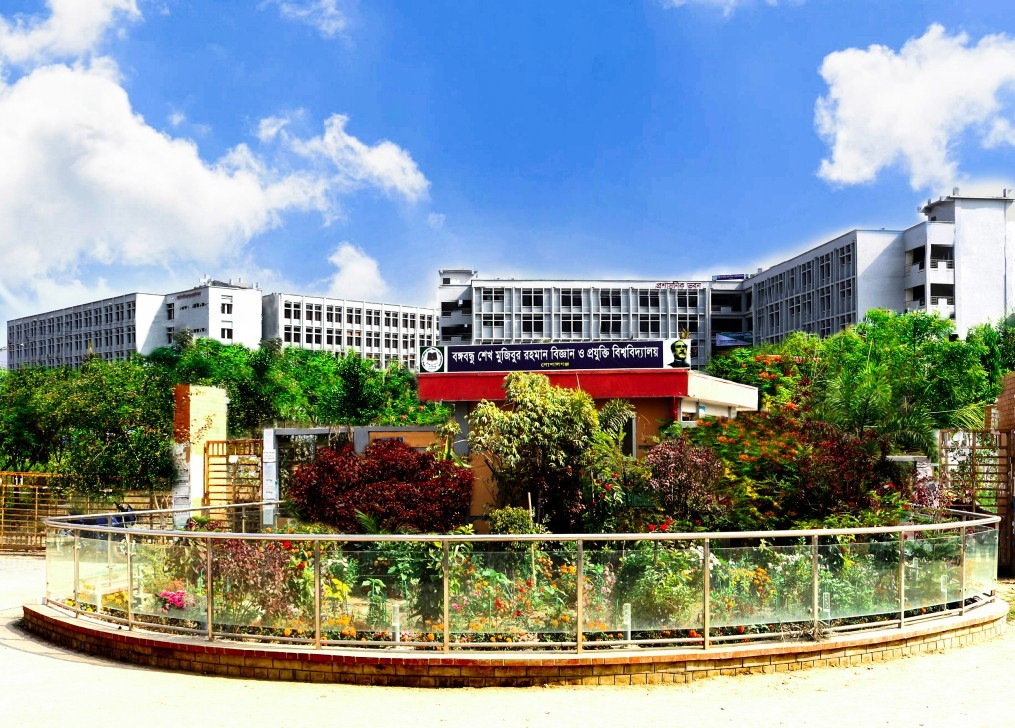
\includegraphics[height=\paperheight,width=\paperwidth]{bsmrstu.jpg}}}
\frame
{
	\titlepage
}
}

% SECTION DEMO

% SECTION 1
\section{Preamble}


%%%%%%%%%%%%%%%%%%%%%%%%%%%%%%%%%%%%%%%%%%%%%%%%%%%%%%%%%%%%%%%%%%%%%%%%
\begin{frame}
	\frametitle{Team Members}
	\begin{tikzpicture}
		\node[draw, text width=5cm, align=center] at (0, 0) {Dr. Saleh Ahmed\\Supervisor\\Associate Professor\\Department of CSE.};
	  \end{tikzpicture}

\end{frame}
%%%%%%%%%%%%%%%%%%%%%%%%%%%%%%%%%%%%%%%%%%%%%%%%%%%%%%%%%%%%%%%%%%%%%%%%


%%%%%%%%%%%%%%%%%%%%%%%%%%%%%%%%%%%%%%%%%%%%%%%%%%%%%%%%%%%%%%%%%%%%%%%%
\begin{frame}
	\frametitle{Start-UP}
	\begin{center}
		Name: Md. Kazi Iqbal Hossen\\
		ID: 18ICTCSE065\\
		Department of CSE\\
		SHIICT, BSMRSTU\\
		\textcolor{green}{\rule{11 cm}{3 pt}} \\

		{\footnotesize \awesomebox[yellow][][]{2pt}{\faExclamationCircle}{red}{This presentation is created and animated with \LaTeX{}-Beamer. Please keep it in full-screen view mode to obtain a better experience.}}
	\end{center}
	\vfill
	\texttt{To obtain beamer source code, click to:}
	\begin{itemize}
		\item[Link 1:] \href{https://pastebin.ubuntu.com/p/dY8TWXY24C/}{\textit{\textbf{Ubuntu pastebin}}}
		\item[Link 2:] \href{https://github.com/Sofiullah-Iqbal-Kiron/LaTeX/blob/master/Presentation/Beamer/MAT205\%20Mid/MAT205\%20Mid.tex}{\textit{\textbf{Github}}}{\tiny (recommended)}
	\end{itemize}
	Or, scan{\footnotesize(clickable in pdf)} the following quick response code:
	\begin{figure}
		\qrcode[hyperlink, padding, height=10mm, level=H, version=8]{https://github.com/Sofiullah-Iqbal-Kiron/LaTeX/blob/master/Presentation/Beamer/MAT205\%20Mid/MAT205\%20Mid.tex}
		\caption*{QR} % package caption
		\centering
	\end{figure}
	\transsplitverticalout[duration=2]
\end{frame}
%%%%%%%%%%%%%%%%%%%%%%%%%%%%%%%%%%%%%%%%%%%%%%%%%%%%%%%%%%%%%%%%%%%%%%%%


% SECTION 2
\section{Basic Beyond}


%%%%%%%%%%%%%%%%%%%%%%%%%%%%%%%%%%%%%%%%%%%%%%%%%%%%%%%%%%%%%%%%%%%%%%%%
\begin{frame}
	\frametitle{Basic Beyond}
	\framesubtitle{What is Fourier series}
	\begin{block}{Fourier Series}
		FS is a special trigonometric periodic series derived by Joseph Fourier$(1768 \rightarrow 1830)$.
	\end{block}

\end{frame}
%%%%%%%%%%%%%%%%%%%%%%%%%%%%%%%%%%%%%%%%%%%%%%%%%%%%%%%%%%%%%%%%%%%%%%%%


%%%%%%%%%%%%%%%%%%%%%%%%%%%%%%%%%%%%%%%%%%%%%%%%%%%%%%%%%%%%%%%%%%%%%%%%
\begin{frame}
	\frametitle{Basic Beyond}
	\framesubtitle{Fourier series: Mathematical Representation}
	Our basic trigonometric series is:
	$$\frac{A_0}{2} + \sum_{n=1}^{\infty} (A_n\cos nx + B_n\sin nx)$$
	It will called \textbf{Fourier Series} if the terms $A_0, A_n, B_n$ is:
	$$A_0 = \frac{1}{2\pi}\int_{-\pi}^{\pi} f(x)\cdot dx$$
	$$A_n = \frac{1}{\pi}\int_{-\pi}^{\pi} f(x)\cdot \cos nx\cdot dx$$
	$$B_n = \frac{1}{\pi}\int_{-\pi}^{\pi} f(x)\cdot \sin nx\cdot dx$$
	Where \textbf{$f(x)$} is any single-valued function defined in interval $(-\pi, \pi)$.
	\sound[autostart, samplingrate=22050]{}{audio.mp3}
	\transfade[duration=0.6]
\end{frame}
%%%%%%%%%%%%%%%%%%%%%%%%%%%%%%%%%%%%%%%%%%%%%%%%%%%%%%%%%%%%%%%%%%%%%%%%


%%%%%%%%%%%%%%%%%%%%%%%%%%%%%%%%%%%%%%%%%%%%%%%%%%%%%%%%%%%%%%%%%%%%%%%%
\begin{frame}
	\frametitle{Basic Beyond}
	\framesubtitle{What is Fourier transform}
	\begin{block}{Fourier Transform}
		FT Is a mathematical transform that decomposes functions depending on time or space into functions depending on spatial or temporal frequency such as the expression of a musical chord.
	\end{block}
	\uncover<2->{
		The Fourier transform of a function due to respect of time is a complex valued function of frequency whose magnitude represents the amount of that frequency present in the original function.
	}
	\transwipe[duration=0.6]
\end{frame}
%%%%%%%%%%%%%%%%%%%%%%%%%%%%%%%%%%%%%%%%%%%%%%%%%%%%%%%%%%%%%%%%%%%%%%%%


%%%%%%%%%%%%%%%%%%%%%%%%%%%%%%%%%%%%%%%%%%%%%%%%%%%%%%%%%%%%%%%%%%%%%%%%
\begin{frame}
	\frametitle{Basic Beyond}
	\framesubtitle{Some helpful equations}
	\begin{enumerate}

		\item<+-| alert@+> $\sin 0\degree = \sin \pi = 0$
		\item<+-| alert@+> $\cos 0\degree = \cos 2n\pi = (-1)^{2n} = 1$
		\item<+-| alert@+> $\cos n\pi = (-1)^n$
		\item<+-| alert@+> $\frac{d}{dx} \sin\theta = \cos\theta$
		\item<+-| alert@+> $\frac{d}{dx} \cos\theta = -\sin\theta$
		\item<+-| alert@+> $\int \sin\theta = -\cos\theta$
		\item<+-| alert@+> $\int \cos\theta = \sin\theta$
		\item<+-| alert@+> $\int UV\cdot dx=U\int V\cdot dx+\int \frac{dU}{dx}(\int V\cdot dx)\cdot dx$

			\transfade[duration=0.15]
	\end{enumerate}
\end{frame}
%%%%%%%%%%%%%%%%%%%%%%%%%%%%%%%%%%%%%%%%%%%%%%%%%%%%%%%%%%%%%%%%%%%%%%%%


% SECTION 3
\section{Illustration 1}


%%%%%%%%%%%%%%%%%%%%%%%%%%%%%%%%%%%%%%%%%%%%%%%%%%%%%%%%%%%%%%%%%%%%%%%%
\begin{frame}[fragile]
	\frametitle{Question 1}
	\begin{block}{1}
		Use the method of Fourier transform to determine the displacement $y(x, t)$ of an infinite string, given that the string is initially at rest and that the initial displacement is $f(x), -\infty < x < \infty$. Also show that the solution can be put in the form:
		\begin{displaymath}
			y(x, t)=\frac{1}{2}\left[f(x+ct)+f(x-ct)\right]
		\end{displaymath}
	\end{block}
	\transwipe[duration=0.6]
\end{frame}
%%%%%%%%%%%%%%%%%%%%%%%%%%%%%%%%%%%%%%%%%%%%%%%%%%%%%%%%%%%%%%%%%%%%%%%%


%%%%%%%%%%%%%%%%%%%%%%%%%%%%%%%%%%%%%%%%%%%%%%%%%%%%%%%%%%%%%%%%%%%%%%%%
\begin{frame}[fragile]
	\frametitle{Question 1}
	\framesubtitle{Trying to solve}
	[Trying to solve:]  \\
	Here we have to solve the one-dimensional wave equation
	$$\frac{\delta^2y}{\delta t^2}=c^2\frac{\delta^2y}{\delta x^2} \hspace{0.5cm}\left[-\infty < x < \infty, t>0\right]$$
	subject to the following initial conditions
	\begin{align*}
		              & y(x,0)=\textrm{Initial displacement}=f(x) \\
		\textrm{and } & y_t(x,0)=\textrm{initial velocity}=0
	\end{align*}
	The given partial differential equation is
	\begin{equation}
		\frac{\delta^2y}{\delta t^2}=c^2\frac{\delta^2y}{\delta x^2}
	\end{equation}
	\transfade[duration=0.6]
\end{frame}
%%%%%%%%%%%%%%%%%%%%%%%%%%%%%%%%%%%%%%%%%%%%%%%%%%%%%%%%%%%%%%%%%%%%%%%%


%%%%%%%%%%%%%%%%%%%%%%%%%%%%%%%%%%%%%%%%%%%%%%%%%%%%%%%%%%%%%%%%%%%%%%%%
\begin{frame}
	\frametitle{Question 1}
	\framesubtitle{Trying to solve}
	Taking the complex Fourier transform of both sides of (1), we have
	\begin{equation}
		\int_{-\infty}^{+\infty}\frac{\delta^2y}{\delta t^2}e^{-iux} dx=c^2\int_{-\infty}^{+\infty}\frac{\delta^2y}{\delta x^2}e^{-iux} dx
	\end{equation}
	By the Fourier transform of the derivative of a function we have if $F^n(x)$ is the nth-derivative of $F(x)$ and the first $(n-1)$ derivatives of F(x) vanish as $x \rightarrow \pm \infty$ then $F\{F^n(x)\}=(-iu)^n F\{F(x)\}$. \\
	Thus from (2) we have
	\begin{align*}
		              & \frac{d^2}{dt^2}\int_{-\infty}^{+\infty}ye^{-iux} dx =c^2(-iu)^2F\{y(x,t)\}                                                                                                       \\
		\textrm{or, } & \frac{d^2}{dt^2}\int_{-\infty}^{+\infty}y(x,t)e^{-iux} dx =c^2(-u^2) F\{y(x,t)\}                                                                                                  \\
		\textrm{or, } & \frac{d^2}{dt^2}F\{y(x,t)\} =-c^2u^2 F\{y(x,t)\}                                                                                                                                  \\
		\textrm{or, } & \frac{d^2\overline{y}}{dt^2} =-c^2u^2\overline{y} \hspace{0.35cm}\left[\textrm{where }\overline{y}=\overline{y}(u,t)=F\{y(x,t)\}=\int_{-\infty}^{+\infty}y(x,t)e^{-iux} dx\right]
	\end{align*}
	\transwipe[duration=0.6]
\end{frame}
%%%%%%%%%%%%%%%%%%%%%%%%%%%%%%%%%%%%%%%%%%%%%%%%%%%%%%%%%%%%%%%%%%%%%%%%


%%%%%%%%%%%%%%%%%%%%%%%%%%%%%%%%%%%%%%%%%%%%%%%%%%%%%%%%%%%%%%%%%%%%%%%%
\begin{frame}[fragile]
	\frametitle{Question 1}
	\framesubtitle{Trying to solve}
	\begin{equation}
		\therefore\hspace{0.5cm}\frac{d^2\overline{y}}{dt^2}+c^2u^2\overline{y}=0
	\end{equation}
	Which is ordinary second order differential equation whose solution is
	\begin{equation}
		\overline{y}=\overline{y}(u,t)=A\cos (cut) + B\sin (cut)
	\end{equation}
	Differentiating with both sides with respect to t
	\begin{equation}
		\textrm{we get, } \overline{y}_t(u,t) = -Acu\sin (cut) + Bcu \cos (cut)
	\end{equation}
	Also from the initial given conditions, we have
	\begin{align}
		 & y(x,0)=f(x) \\
		 & y_t(x,0)=0
	\end{align}
	\transfade[duration=0.6]
\end{frame}
%%%%%%%%%%%%%%%%%%%%%%%%%%%%%%%%%%%%%%%%%%%%%%%%%%%%%%%%%%%%%%%%%%%%%%%%


%%%%%%%%%%%%%%%%%%%%%%%%%%%%%%%%%%%%%%%%%%%%%%%%%%%%%%%%%%%%%%%%%%%%%%%%
\begin{frame}[fragile]
	\frametitle{Question 1}
	\framesubtitle{Trying to solve}
	Taking the Fourier transform of (6) and (7) we get,
	$$\overline{y}(u,0)=\int_{-\infty}^{+\infty}y(x,0)e^{-iux}\cdot dx=\int_{-\infty}^{+\infty}f(x)e^{-iux}\cdot dx=\overline{f}(u)\hspace{0.3cm} \textrm{(say)} $$
	\begin{equation}
		\therefore\hspace{0.5cm}\overline{y}(u,0)=\overline{f}(u)
	\end{equation}
	\begin{align*}
		\textrm{and } \overline{y}_t(u,0) & =\int_{-\infty}^{+\infty}y_t(x,0)e^{-iux}\cdot dx \\
		                                  & =\int_{-\infty}^{+\infty}0(e^{-iux})\cdot du=0
	\end{align*}
	\begin{equation}
		\therefore \hspace{0.3cm}\overline{y}_t(u,0)=0
	\end{equation}
	Putting t = 0 in (5), we have $\overline{y}_t(u,0)=Bcu$ \\
	or, $Bcu=0$ using (9) \\
	\hspace{2cm}$\therefore\hspace{0.5cm} B=0 \hspace{0.5cm} \textrm{Since, }cu \neq 0$ \\
	\transwipe[duration=0.6]
\end{frame}
%%%%%%%%%%%%%%%%%%%%%%%%%%%%%%%%%%%%%%%%%%%%%%%%%%%%%%%%%%%%%%%%%%%%%%%%


%%%%%%%%%%%%%%%%%%%%%%%%%%%%%%%%%%%%%%%%%%%%%%%%%%%%%%%%%%%%%%%%%%%%%%%%
\begin{frame}[fragile]
	\frametitle{Question 1}
	\framesubtitle{Trying to solve}
	Again putting t = 0 in (4), we get
	\begin{align*}
		                          & \overline{y}(u,0)=A                                 \\
		\therefore \hspace{0.3cm} & \overline{f}(u)=A \hspace{0.5cm} \textrm{using (8)} \\
		\textrm{or, }             & A=\overline{f}(u)
	\end{align*}
	Putting the values of A and B in (4), we get
	\begin{equation}
		\overline{y}=\overline{y}(u,t)=\overline{f}(u)\cos (cut)
	\end{equation}
	Taking the inverse Fourier transform of (10) we have
	\begin{align*}
		              & y(x,t)=\frac{1}{2\pi}\int_{-\infty}^{+\infty}\overline{f}(u)\cos (cut)e^{iux}\cdot du                                                                                                      \\
		\textrm{or, } & y(x,t)=\frac{1}{2\pi}\int_{-\infty}^{+\infty}\overline{f}(u)\left(\frac{e^{icut}+e^{-icut}}{2}\right) e^{iux}\cdot du                                                                      \\
		              & \hspace{1cm}=\frac{1}{2}\left[\frac{1}{2\pi}\int_{-\infty}^{+\infty}\overline{f}(u)e^{iu(x+ct)}\cdot du + \frac{1}{2\pi}\int_{-\infty}^{+\infty}\overline{f}(u)e^{iu(x-ct)}\cdot du\right] \\
		              & \hspace{1cm}\mbox{\small $=\frac{1}{2}\left[f(x+ct)+f(x-ct)\right]$}\hspace{0.1cm} \textrm{\scriptsize{(Using the definition of inverse Fourier transform)}}
	\end{align*}
	\transfade[duration=0.6]
\end{frame}
%%%%%%%%%%%%%%%%%%%%%%%%%%%%%%%%%%%%%%%%%%%%%%%%%%%%%%%%%%%%%%%%%%%%%%%%


%%%%%%%%%%%%%%%%%%%%%%%%%%%%%%%%%%%%%%%%%%%%%%%%%%%%%%%%%%%%%%%%%%%%%%%%
\begin{frame}[fragile]
	\frametitle{Question 1}
	\framesubtitle{Solved}
	\begin{block}{Finally}
		$\therefore\hspace{0.5cm}y(x,t)=\frac{1}{2}\left[f(x+ct)+f(x-ct)\right]$.
	\end{block}
	\transwipe[duration=0.6]
\end{frame}
%%%%%%%%%%%%%%%%%%%%%%%%%%%%%%%%%%%%%%%%%%%%%%%%%%%%%%%%%%%%%%%%%%%%%%%%


% SECTION 4
\section{Illustration 2}


%%%%%%%%%%%%%%%%%%%%%%%%%%%%%%%%%%%%%%%%%%%%%%%%%%%%%%%%%%%%%%%%%%%%%%%%
\begin{frame}[fragile]
	\frametitle{Question 2}
	\begin{block}{2}
		A thin membrane of great extent is released from rest in the position $z=f(x,y)$, show that the displacement at any subsequent time is given by
		$$z(x,y,t)=\frac{1}{2\pi}\int_{-\infty}^{+\infty}\int_{-\infty}^{+\infty}F(u,v)\cos ct\sqrt{(u^2+v^2)}\cdot e^{-i(ux+vy)}\cdot du\cdot dv$$
		where $F(u,v)$ is the double Fourier transform of $f(x,y)$.
	\end{block}
	\transfade[duration=0.6]
\end{frame}
%%%%%%%%%%%%%%%%%%%%%%%%%%%%%%%%%%%%%%%%%%%%%%%%%%%%%%%%%%%%%%%%%%%%%%%%


%%%%%%%%%%%%%%%%%%%%%%%%%%%%%%%%%%%%%%%%%%%%%%%%%%%%%%%%%%%%%%%%%%%%%%%%
\begin{frame}[fragile]
	\frametitle{Question 2}
	\framesubtitle{Trying to proof}
	[Trying to proof:] \\
	Here the displacement of the membrane is governed by two dimensional wave equation
	\begin{equation} \tag{1}
		\frac{\delta^2z}{\delta t^2}=c^2\left(\frac{\delta^2z}{\delta x^2}+\frac{\delta^2z}{\delta y^2}\right) \hspace{0.5cm}\textrm{where }c^2=\frac{T}{\rho}
	\end{equation}
	Taking the double Fourier transform of both sides of (1) we get
		{\small
			\begin{displaymath}
				\Rightarrow\frac{1}{2\pi}\int_{-\infty}^{+\infty}\int_{-\infty}^{+\infty}\frac{\delta^2z}{\delta t^2}e^{i(ux=vy)}\cdot dx\cdot dy = \frac{c^2}{2\pi}\int_{-\infty}^{+\infty}\int_{-\infty}^{+\infty}\left(\frac{\delta^2z}{\delta x^2}+\frac{\delta^2z}{\delta y^2}\right)e^{i(ux+vy)}\cdot dx\cdot dy
			\end{displaymath}
		}
	\begin{multline*}
		\textrm{or, } \frac{d^2}{dt^2} \frac{1}{2\pi}\int_{-\infty}^{+\infty}\int_{-\infty}^{+\infty}ze^{i(ux+vy)}\cdot dx\cdot dy= \\ \frac{c^2}{2\pi}\int_{-\infty}^{+\infty}\int_{-\infty}^{+\infty}\left(\frac{\delta^2z}{\delta x^2}+\frac{\delta^2z}{\delta y^2}\right)e^{i(ux+vy)}\cdot dx\cdot dy
	\end{multline*}
	\transwipe[duration=0.6]
\end{frame}
%%%%%%%%%%%%%%%%%%%%%%%%%%%%%%%%%%%%%%%%%%%%%%%%%%%%%%%%%%%%%%%%%%%%%%%%


%%%%%%%%%%%%%%%%%%%%%%%%%%%%%%%%%%%%%%%%%%%%%%%%%%%%%%%%%%%%%%%%%%%%%%%%
\begin{frame}[fragile]
	\frametitle{Question 2}
	\framesubtitle{Trying to proof}
	\begin{multline*}
		\textrm{or,} \frac{d^2\overline{z}}{dt^2}=c^2\{(-iu)^2+(-iv)^2\} F\{z(x,y,t)\}\textrm{    where } \overline{z}=\overline{z}(u,v,t)=F\{z(x,y,t)\}\\=\frac{1}{2\pi}\int_{-\infty}^{+\infty}\int_{-\infty}^{+\infty}ze^{i(ux+vy)}\cdot dx\cdot dy
	\end{multline*}
	\begin{flalign*}
		\hspace{0.35cm}\textrm{or, }\frac{d^2\overline{z}}{dt^2}=-c^2(u^2+v^2)\overline{z} &  & % double amper sign (&&) after equation in flalign environment is required to make it left align.
	\end{flalign*}
	\begin{equation}\tag{2}
		\therefore\hspace{0.5cm}\frac{d^2\overline{z}}{dt^2}+c^2(u^2+v^2)\overline{z}=0
	\end{equation}
	\transfade[duration=0.6]
\end{frame}
%%%%%%%%%%%%%%%%%%%%%%%%%%%%%%%%%%%%%%%%%%%%%%%%%%%%%%%%%%%%%%%%%%%%%%%%


%%%%%%%%%%%%%%%%%%%%%%%%%%%%%%%%%%%%%%%%%%%%%%%%%%%%%%%%%%%%%%%%%%%%%%%%
\begin{frame}[fragile]
	\frametitle{Question 2}
	\framesubtitle{Trying to proof}
	which is an ordinary differential equation whose solution is
	\begin{equation}\tag{3}
		\overline{z}=A\cos\{c\sqrt{(u^2+v^2)}t\}+B\sin\{c\sqrt{(u^2+v^2)}t\}
	\end{equation}
	The given initial conditions are $\overline{z}=f(x,y) \textrm{ and }\frac{\delta z}{\delta t}=0 \textrm{ at }t=0$ \\
	Taking the Fourier transform of these initial conditions, we get
	\begin{equation}\tag{4}
		\overline{z}=\frac{1}{2\pi}\int_{-\infty}^{+\infty}\int_{-\infty}^{+\infty}f(x,y)e^{i(ux+vy)}\cdot dx\cdot dy=F(u,v)
	\end{equation}
	\begin{flalign*}
		 & =\frac{1}{2\pi}\int_{-\infty}^{+\infty}\int_{-\infty}^{+\infty}\frac{\delta z}{\delta t}e^{i(ux+vy)}\cdot dx\cdot dy                                 &  & \\
		 & =\frac{d}{dt}\frac{1}{2\pi}\int_{-\infty}^{+\infty}\int_{-\infty}^{+\infty}ze^{i(ux+vy)}\cdot dx\cdot dy                                             &  & \\
		 & =\frac{d\overline{z}}{dt} \textrm{  since  }\overline{z}=\frac{1}{2\pi}\int_{-\infty}^{+\infty}\int_{-\infty}^{+\infty}ze^{i(ux+vy)}\cdot dx\cdot dy &  &
	\end{flalign*}
	\transwipe[duration=0.6]
\end{frame}
%%%%%%%%%%%%%%%%%%%%%%%%%%%%%%%%%%%%%%%%%%%%%%%%%%%%%%%%%%%%%%%%%%%%%%%%


%%%%%%%%%%%%%%%%%%%%%%%%%%%%%%%%%%%%%%%%%%%%%%%%%%%%%%%%%%%%%%%%%%%%%%%%
\begin{frame}[fragile]
	\frametitle{Question 2}
	\framesubtitle{Trying to proof}
	\begin{flalign*}
		\therefore\hspace{0.5cm}\frac{d\overline{z}}{dt}=0 \textrm{  at  }t=0 &  &
	\end{flalign*}
	When t=0, combining (3) and (4), we get $A=F(u,v)$
	\begin{flalign*}
		\textrm{Also }           & \frac{d\overline{z}}{dt}=-Ac\sqrt{(u^2+v^2)}\sin c\sqrt{(u^2+v^2)t}+Bc\sqrt{(u^2+v^2)}\cos c\sqrt{(u^2+v^2)}t &  & \\
		\therefore\hspace{0.2cm} & 0=\left(\frac{d\overline{z}}{dt}\right)_{t=0}=Bc\sqrt{(u^2+v^2)}                                              &  & \\
		\textrm{or, }            & B=0
	\end{flalign*}
	Putting the values of A and B in (3), we get
	\begin{equation}\tag{5}
		\overline{z}=F(u,v)cos\{c\sqrt{(u^2+v^2)t}\}
	\end{equation}
	\transfade[duration=0.6]
\end{frame}
%%%%%%%%%%%%%%%%%%%%%%%%%%%%%%%%%%%%%%%%%%%%%%%%%%%%%%%%%%%%%%%%%%%%%%%%


%%%%%%%%%%%%%%%%%%%%%%%%%%%%%%%%%%%%%%%%%%%%%%%%%%%%%%%%%%%%%%%%%%%%%%%%
\begin{frame}[fragile]
	\frametitle{Question 2}
	\framesubtitle{Proved}
	\begin{block}{Ultimately}
		Now applying the inversion formula for double Foruier transform, we have
		$$z(x,y,t)=\frac{1}{2\pi}\int_{-\infty}^{+\infty}\int_{-\infty}^{+\infty}F(u,v)\cos \{c\sqrt{(u^2+v^2)}t\}e^{-i(ux+vy)}\cdot du\cdot dv$$
		Which is the required displacement at any subsequent time t.
	\end{block}
	\transwipe[duration=0.6]
\end{frame}
%%%%%%%%%%%%%%%%%%%%%%%%%%%%%%%%%%%%%%%%%%%%%%%%%%%%%%%%%%%%%%%%%%%%%%%%


% SECTION 5
\section{Ending Scene}


%%%%%%%%%%%%%%%%%%%%%%%%%%%%%%%%%%%%%%%%%%%%%%%%%%%%%%%%%%%%%%%%%%%%%%%%
%\begin{frame}
%\frametitle{Issues}
%\end{frame}
%%%%%%%%%%%%%%%%%%%%%%%%%%%%%%%%%%%%%%%%%%%%%%%%%%%%%%%%%%%%%%%%%%%%%%%%


%%%%%%%%%%%%%%%%%%%%%%%%%%%%%%%%%%%%%%%%%%%%%%%%%%%%%%%%%%%%%%%%%%%%%%%%
\begin{frame}[fragile]
	\begin{block}{EOF}
		End Of File.
	\end{block}
	\transfade[duration=0.6]
\end{frame}
%%%%%%%%%%%%%%%%%%%%%%%%%%%%%%%%%%%%%%%%%%%%%%%%%%%%%%%%%%%%%%%%%%%%%%%%


\end{document}
